%==============================
\subsection{Simulations and Experiment}\label{subsec:simulation}


The numerical study simulates a team of multiple UGVs and UAVs
that are responsible for maintaining a remote photovoltaic (PV) power station.
We first describe the scenario and three types of tasks,
followed by the results obtained via the proposed method.
Then, we introduce various changes in the environment and agent failures,
in order to validate the proposed online adaptation algorithm.
Third, we perform scalability analysis of our method by increasing
the system size and the task complexity.
Lastly, we compare our methods against several strong baselines, in terms of
optimality, computation time and adaptation efficiency.


%==============================
\begin{figure}
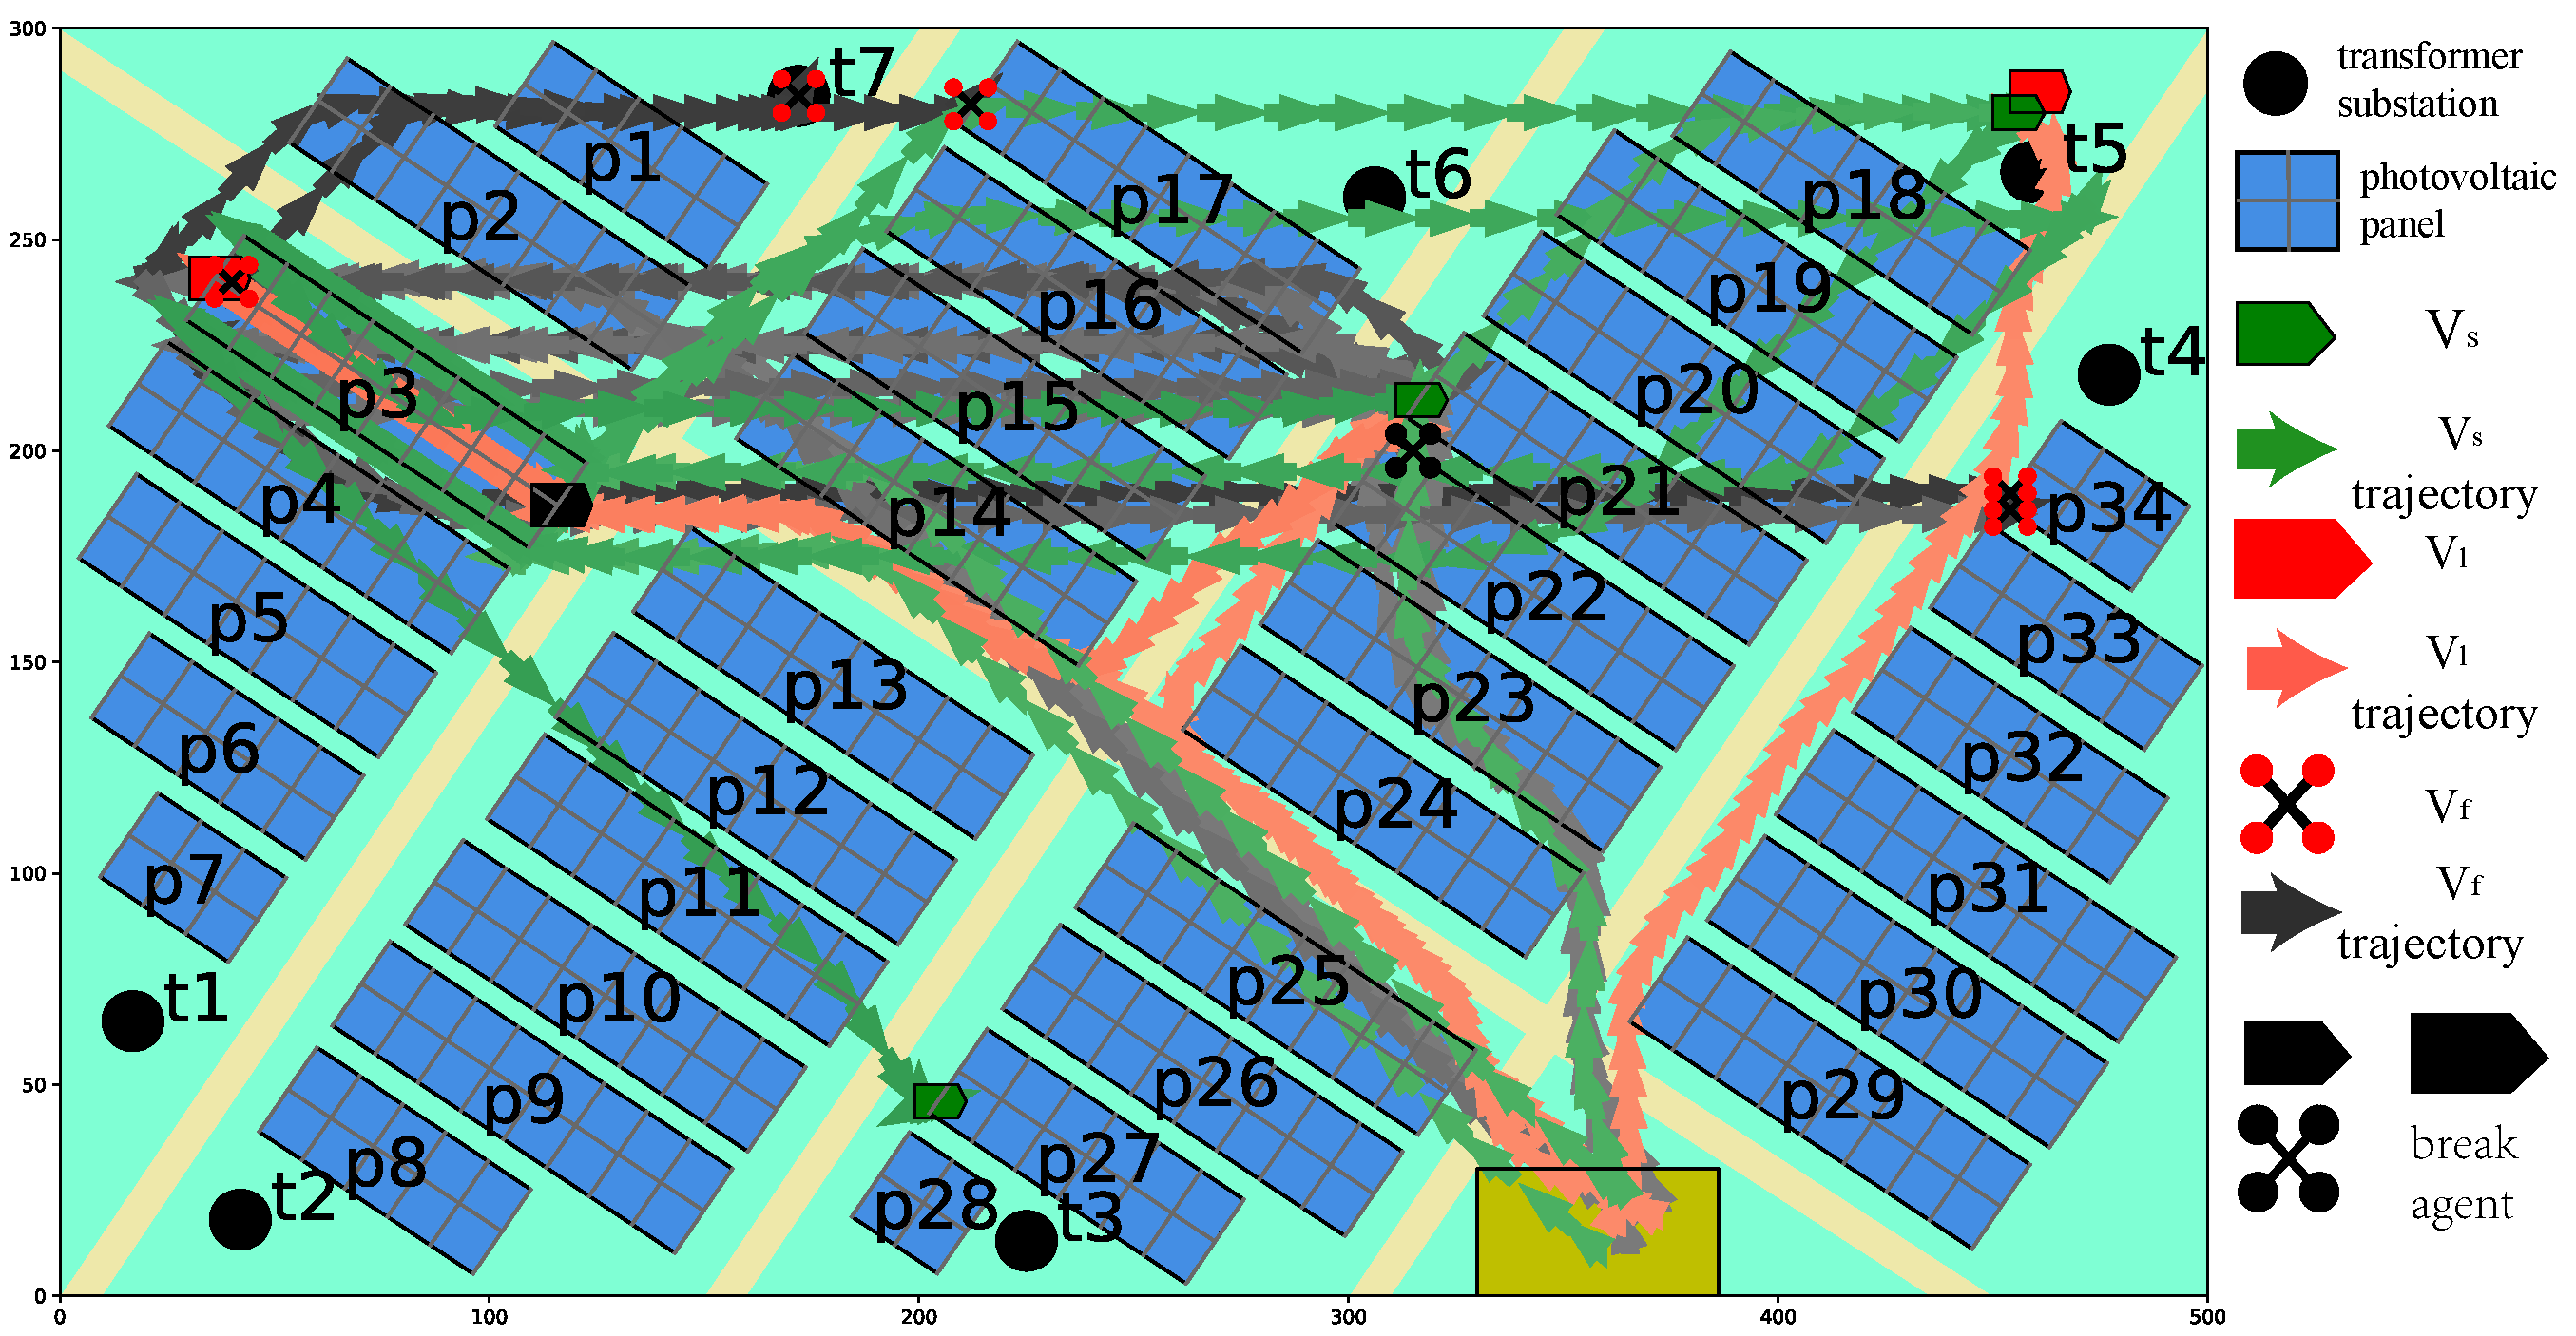
\includegraphics[scale=0.18]{figures/background3.pdf}
\caption{Simulated PV power station in the numerical study,
  which consists of PV panels~$\texttt{p}_i$, roads,
  inverters/transformers~$\texttt{t}_i$ and base stations~$b$.
  The arrow trajectories are the path of Agent swarm
  executing the LTL formula~$\varphi_{3}$. And the arrow direction
  is the motion direction and the arrow density correspond to the velocity of different agents.}
\label{fig:workspace}
\end{figure}
%==============================

%==============================
\subsubsection{Workspace Description}\label{subsubsec:ws}

Consider a group of UAVs and UGVs that work within a PV power station for
long-term daily maintenance.
As shown in Fig.~\ref{fig:workspace},
the station consists of mainly three parts: PV panels $\texttt{p}_1,\cdots,\texttt{p}_{34}$, roads,
inverter/transformer substations $\texttt{t}_1,\cdots,\texttt{t}_7$ and the robot base station $\texttt{b}$. 
Furthermore, there are one type of UAVs and two types of UGVs as table~\ref{table:agent} showed.
The UAVs $V_f$ are quadcopters which can move freely between all interested places.
The larger type of UGVs, denoted by $V_l$, has the limitation of not going to PV panels or transformers;
the smaller ones $V_s$ can travel more freely, e.g., under the PV panels but not under the transformers. 
As a result, different types of robots have different motion 
model~$\mathcal{G}_n$ as described in Sec.~\ref{subsec:multi-agent}
and distinctive action models.
The traveling time among the regions of interest is estimated by the route
distance and their respective speed. The actions required and the  
Descriptions of these regions of interest and robot actions are summarized in
Table.~\ref{fig:symbols}.
Note that some actions can be performed alone while some require direct
collaboration of several agents,
e.g., one $V_s$ can $sweep$ debris under the PV panel while one $V_l$
and two $V_s$ are required to $repair$ a broken PV panel.


%==============================
\subsubsection{Task Description}\label{subsubsec:task}

For the nominal scenario, we consider a system of moderate size,
including $12$ agents: 6 $V_f$, 3 $V_l$ and 3 $V_s$.
Scalability analysis to larger systems are performed later in Sec.~\ref{subsubsec:scalable}.
Moreover, we consider a complex task and test it with agent failure.

\begin{table}[t]
\caption{definition of agent with function}
\label{table:agent}
\begin{tabular}{|c|c |c|c|}\hline
	\textbf{Agent type} &\textbf{label} & \textbf{Capable action} & \textbf{Speed}$(m/ s )$\\ \hline
	 Quadcopter& $V_f$  & $temp, scan, wash $ & 10 \\ \hline
	 Larger UGV& $V_l$  & $wash,repair_l,fix$ & 4 \\ \hline
	 Smaller UGV& $V_s$  &  $sweep, mow, repair_s, fix$ & 4 \\ \hline
\end{tabular}
\end{table}


%==============================
\begin{table}[t]
 \centering
\caption{Description of related regions and agent actions.}
\label{fig:symbols}
\begin{tabular}{|c|m{0.5\columnwidth}|c|}\hline
\textbf{Proposition} & \textbf{Description}\centering & \textbf{Duration} [s]\\ \hline
$\texttt{p}_1,\cdots,\texttt{p}_{34}$ & $34$ PV panels. & $\backslash$ \\ \hline
$\texttt{b}$ & Base stations for all agents to park and charge. & $\backslash$ \\ \hline
$\texttt{t}_1,\cdots,\texttt{t}_7$ & $7$ transformers. & $\backslash$ \\ \hline
$\texttt{temp}_{\texttt{p}_i,\texttt{t}_i}$ &
Measure temperature of panel~$\texttt{p}_i$ and transformer $\texttt{t}_i$.
Requires 1 $temp$ action. & 10 \\ \hline
$\texttt{sweep}_{\texttt{p}_i}$& Sweep debris around any panel~$\texttt{p}_i$.
Requires 1 $sweep$ action. & 190\\ \hline
$\texttt{mow}_{\texttt{p}_i,\texttt{t}_i}$ &
Mow the grass under panel~$\texttt{p}_i$ or transformer~$\texttt{t}_i$.
Requires 1 $mow$ action. & 190\\ \hline
$\texttt{fix}_{\texttt{t}_i}$ &
Fix malfunctional transformer~$\texttt{t}_i$.
Requires 2 $fix$ action collaborations & 72\\ \hline
$\texttt{repair}_{\texttt{p}_i}$ &
Repair broken panel~$\texttt{p}_i$.
Requires 2 $repair_s$,1 $repair_l$ action collaborations . & 576\\ \hline
$\texttt{wash}_{\texttt{p}_i}$ &
Wash the dirt off panel~$\texttt{p}_i$.
Requires 2 $wash$ actions collaborations. & 565\\ \hline
$\texttt{scan}_{\texttt{p}_i,\texttt{t}_i}$ &
Build 3D models of panel~$\texttt{p}_i$ or transformer~$\texttt{t}_i$
for inspection. Requires 3 $scan$ action. & 95\\ \hline
\end{tabular}
\end{table}
%==============================

This task can be specified as the following LTL formulas, 
requires a series of limited actions to 
maintain the photovoltaic power station:
\begin{equation}\label{eq:task1}
  \begin{aligned}
\varphi_1 = & \Diamond(\texttt{repair}_{\texttt{p}_{3}} \wedge \lnot \texttt{scan}_{\texttt{p}_3} \wedge\Diamond \texttt{scan}_{\texttt{p}_3})
\wedge \Diamond (\texttt{wash}_{\texttt{p}_{21}} \wedge \\
&\Diamond \texttt{mow}_{\texttt{p}_{21}} \wedge \Diamond \texttt{scan}_{\texttt{p}_{21}}) \wedge \Diamond ( \texttt{sweep}_{\texttt{p}_{21}} \wedge \lnot \texttt{wash}_{\texttt{p}_{21}} \wedge\\
& \Diamond \texttt{mow}_{\texttt{p}_{21}}) \wedge \Diamond(\texttt{fix}_{\texttt{t}_5} \wedge \lnot \texttt{p}_{\texttt{18}}) \wedge \lnot \texttt{p}_{24} \,U \, \texttt{sweep}_{\texttt{p}_{27}} \\
&\wedge \Diamond (\texttt{wash}_{\texttt{p}_{34}} \wedge \bigcirc \texttt{scan}_{\texttt{p}_{34}})
\end{aligned}
\end{equation}

The location of these subtasks are chosen across the workspace
thus a coordination strategy to minimize completion time is crucial for the task.



%===========================
\begin{figure}[t!] 
		\centering%
		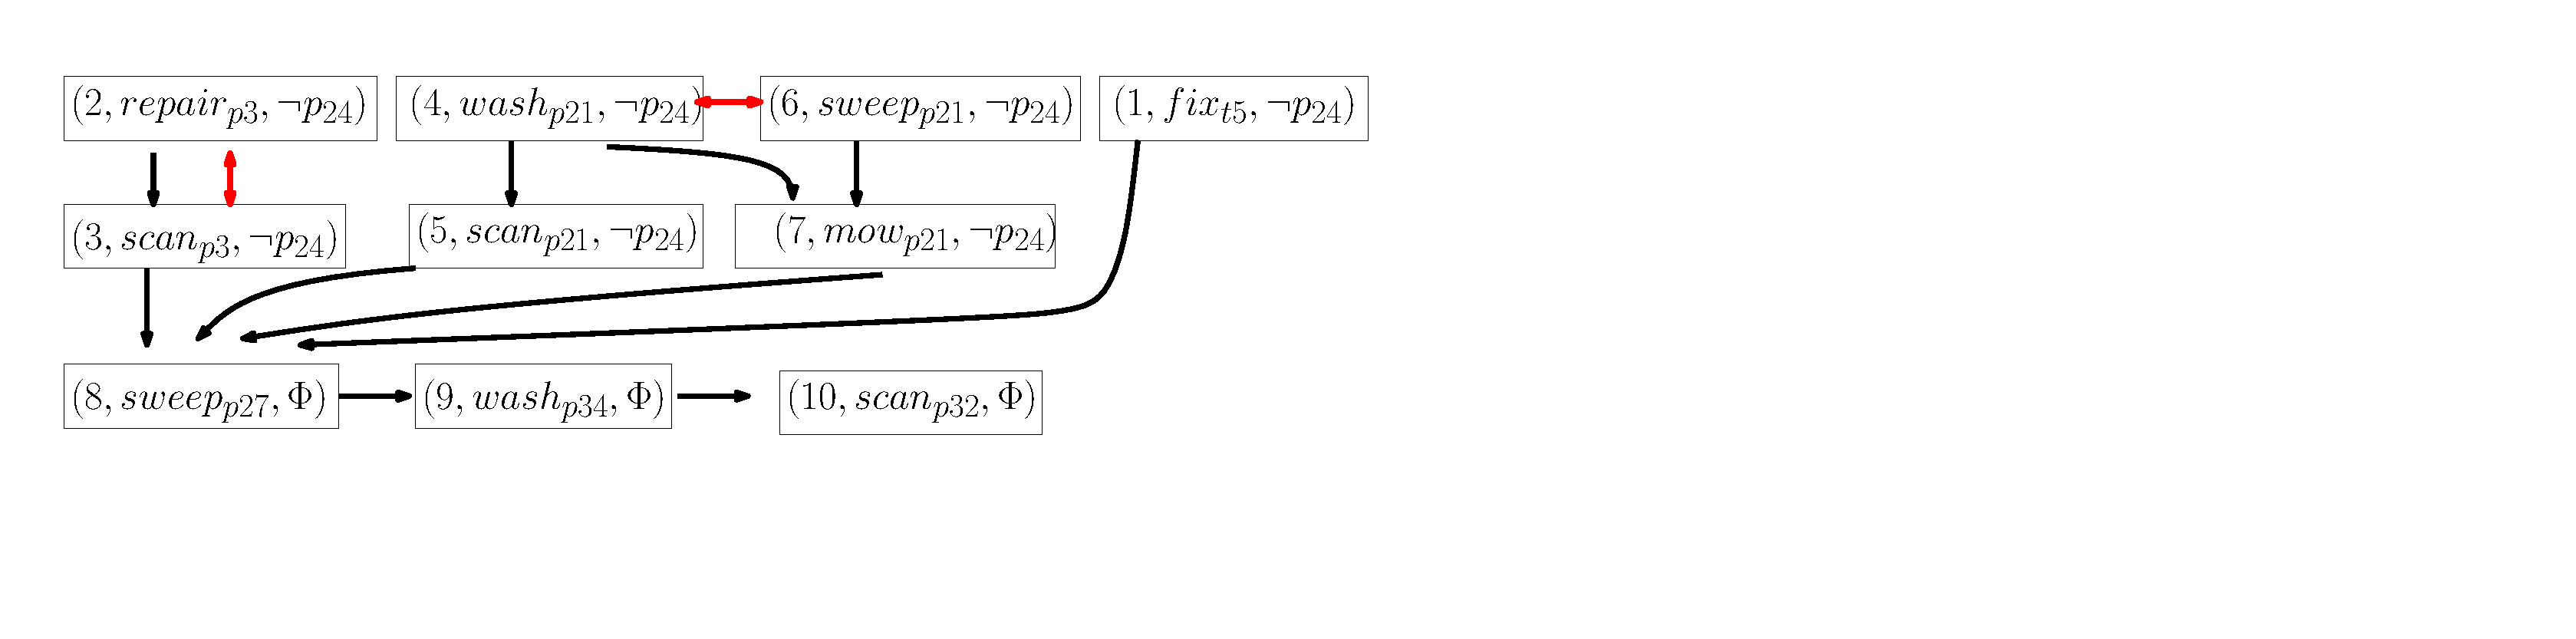
\includegraphics[height = 0.12 \textwidth]{figures/simulation/taskfinal/ipe_poset_graph.pdf}
	\caption{Poset graph of task $\varphi_1$.
          The relations~$\preceq_\varphi,\, \neq_{\varphi}$ are marked
          by black and red arrows, respectively.}
       \label{fig:task12-posets}
\end{figure}
%===========================

%========================================
\subsubsection{Results}\label{subsubsec:results}
In this section, we present the results of the proposed method for
the above tasks, including the computation of posets,
task assignment via the BnB search algorithm, and the task execution results.

\textbf{Partial analysis}:
The NBA~$\mathcal{B}_{\varphi_1}$ associated with task one in~\eqref{eq:task1}
contains~$707$ states and~$16044$ edges. And the pruning step reduced $84.9\%$ edges within 
$30.43$ second. Then, the Alg.~\ref{alg:compute-poset} explores 
 $4$ accepting runs in $0.14s$ to find the first poset and get the one of the best poset in $22.40s$.
 Finally showed in \ref{fig:task12-posets}, we choose the best poset $P^{p}_{\varphi}$ with $10$ subtasks, whose language 
 $L(P^{p}_{\varphi})$ has $525$ \emph{Words}. In $P^{p}_{\varphi}$, there are 
 multiple subtasks can be executed in parallel such as $\omega_2 $ with $ \omega_4$,$\omega_1 $ with $ \omega_7$.
 However, these subtasks are still ordered as no subtask set can be executed independent with the left 
 subtasks. That means we cannot
 divide the word into series independent parts with the method in \cite{schillinger2018simultaneous}.
 It's worth noting this poset has only one subtask $\omega_7$ with $\texttt{mow}_{\texttt{p}_{21}}$,
 which is required in twice in $\varphi_1$. And it follows additions partial orders as
 $\omega_4\leq_\varphi \omega_6,\omega_2\leq_\varphi \omega_6$. That means our method found 
 a more efficient poset with relations not explicitly written in the formula.
 There are two $\neq_\varphi$ relations as $(\omega_1,\omega_3),(\omega_2,\omega_4)$, due to the constrains 
 $\Box(\texttt{repair}_{\texttt{p}_3}\rightarrow\lnot\texttt{scan}_{\texttt{p}_3}) $ and
  $\texttt{sweep}_{\texttt{p}_{21}} \wedge \lnot \texttt{wash}_{\texttt{p}_{21}}$ in formula $\varphi_1$.
  Before execute $\omega_8$, all subtasks has the self-loop constrains $\lnot p_{24}$ due to
   $\lnot \texttt{p} U \texttt{sweep}_{\texttt{p}_{27}}$.
   

%===========================
\begin{figure}[t!]
\centering%
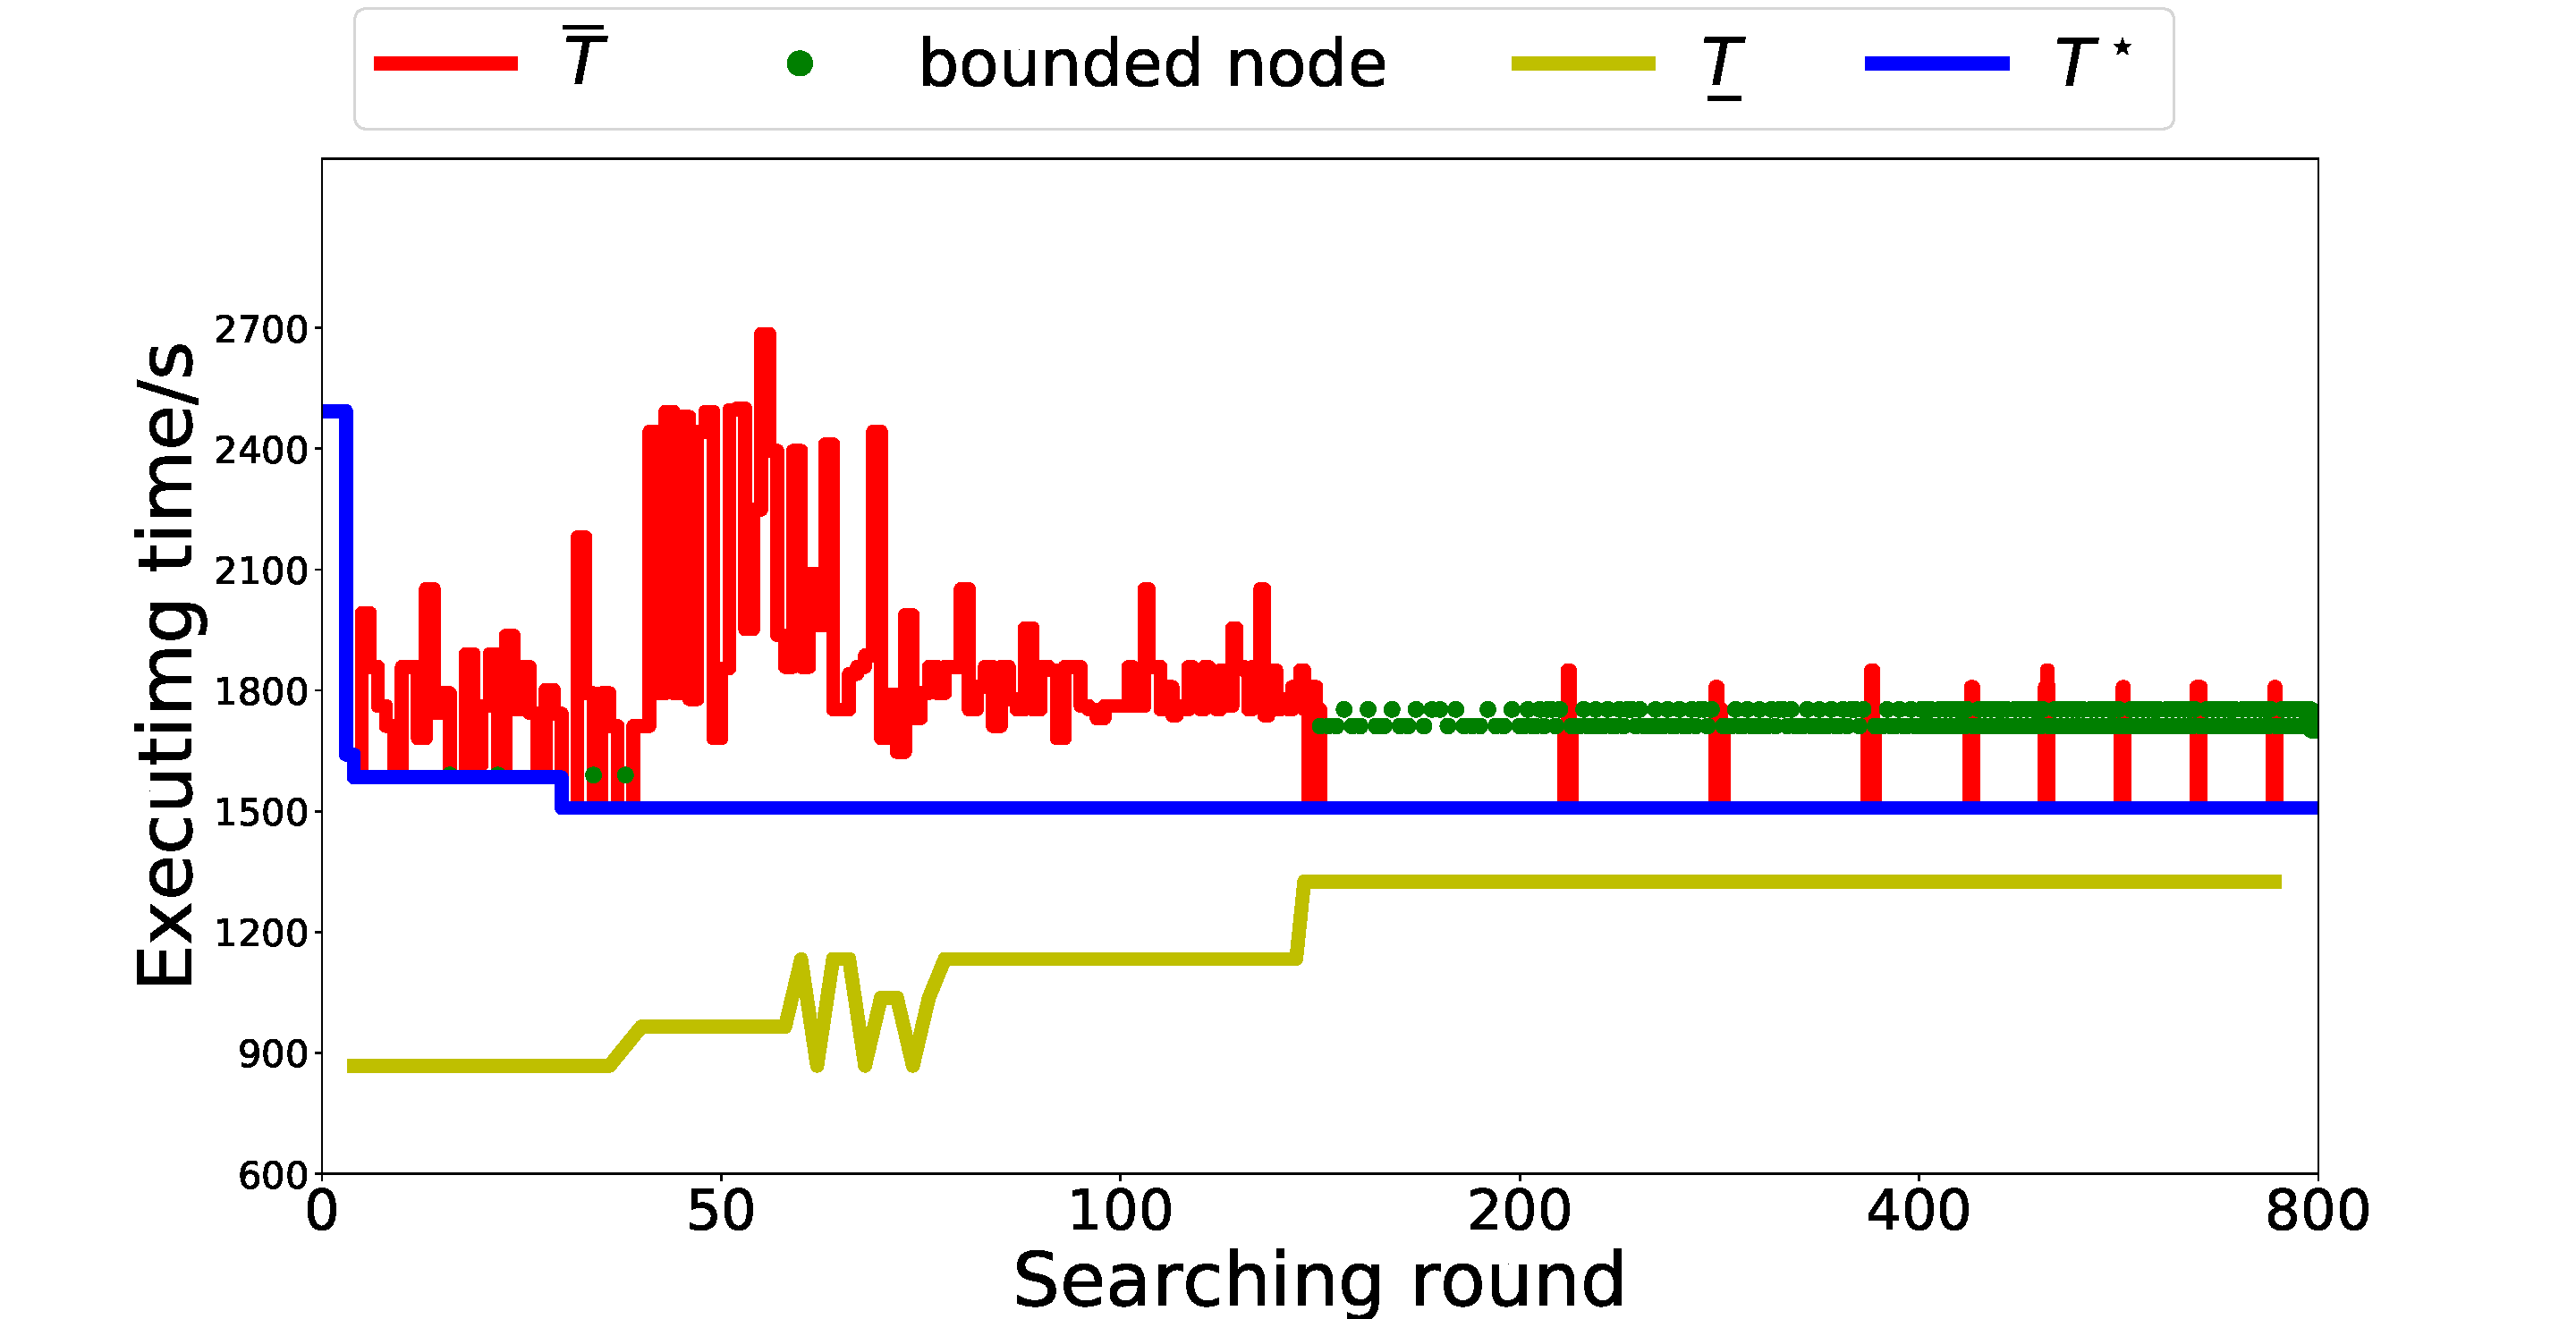
\includegraphics[width = 0.50\textwidth]{figures/simulation/taskfinal/bnb.pdf}
\caption{Illustration of the upper and lower
bounds~$\overline{T}_\nu,\,\underline{T}_\nu$, and the optimal value~$T^\star$,
along with the BnB search process.}
\label{fig:task2-bnb}
\end{figure}
%===========================
\textbf{Task assignment}
Then, during the task assignment step,
the first valid solution is found in~$0.131s$.
Afterwards, at~$t=1.75s$, a node is reached and its estimated lower
bound is larger than current upper bound, and thus cut off the search tree.
Overall, around~$84.2\%$ of visited nodes are cut off,
which clearly shows the benefits of the ``bounding'' mechanism.
Then, the estimated upper-bound rapidly converged
to the optimal $T^\star=1388.5s$ in~$3.34s$ with exploring~$30$ nodes.
This is due to the branching efficiency during the BnB search,
by using the estimated lower bounds as heuristics.
Lastly, the whole search tree is exhausted after more than~$10$ hours
due to the complexity of the problem. 


In the optimal task assignment, for the same type of task $\texttt{wash}$,
different type of agent are employed as $V_{f3},V_{l9}$ for $\texttt{wash}_{\texttt{p}_{21}}$ and
 $V_{f4},V_{f5}$ for $\texttt{wash}_{\texttt{p}_{34}}$. And all the constrains 
 of $\leq_\varphi,\neq_\varphi$ are satisfied such as $\texttt{mow}_{\texttt{p}_{21}}$ 
should be executed after $\texttt{repair}_{\texttt{p}_3}$, $\texttt{sweep}_{\texttt{p}_21}$
should not be execute at same time which denote by triangles of the corresponding color.
What's more, the most subtasks without these relations are executed parallel as $\omega_1,\omega_2$.
These parallelisms dramatically reduce the make span.
In the trajectory graph~\ref{fig:workspace}, the self-loop constrains of each subtasks are all satisfied
as before executing $\omega_8$, no agent is permitted enter the PV panels $P_{24}$, while $V_f, V_s$ are allowed 
crossing other PV panels.
In addition, the assignment of
suffix $P^s_\varphi$ is showed in the lower part of \ref{Gantt_graph}.


%==============================
\begin{figure}[t!]
  \begin{minipage}[t]{1\linewidth}
		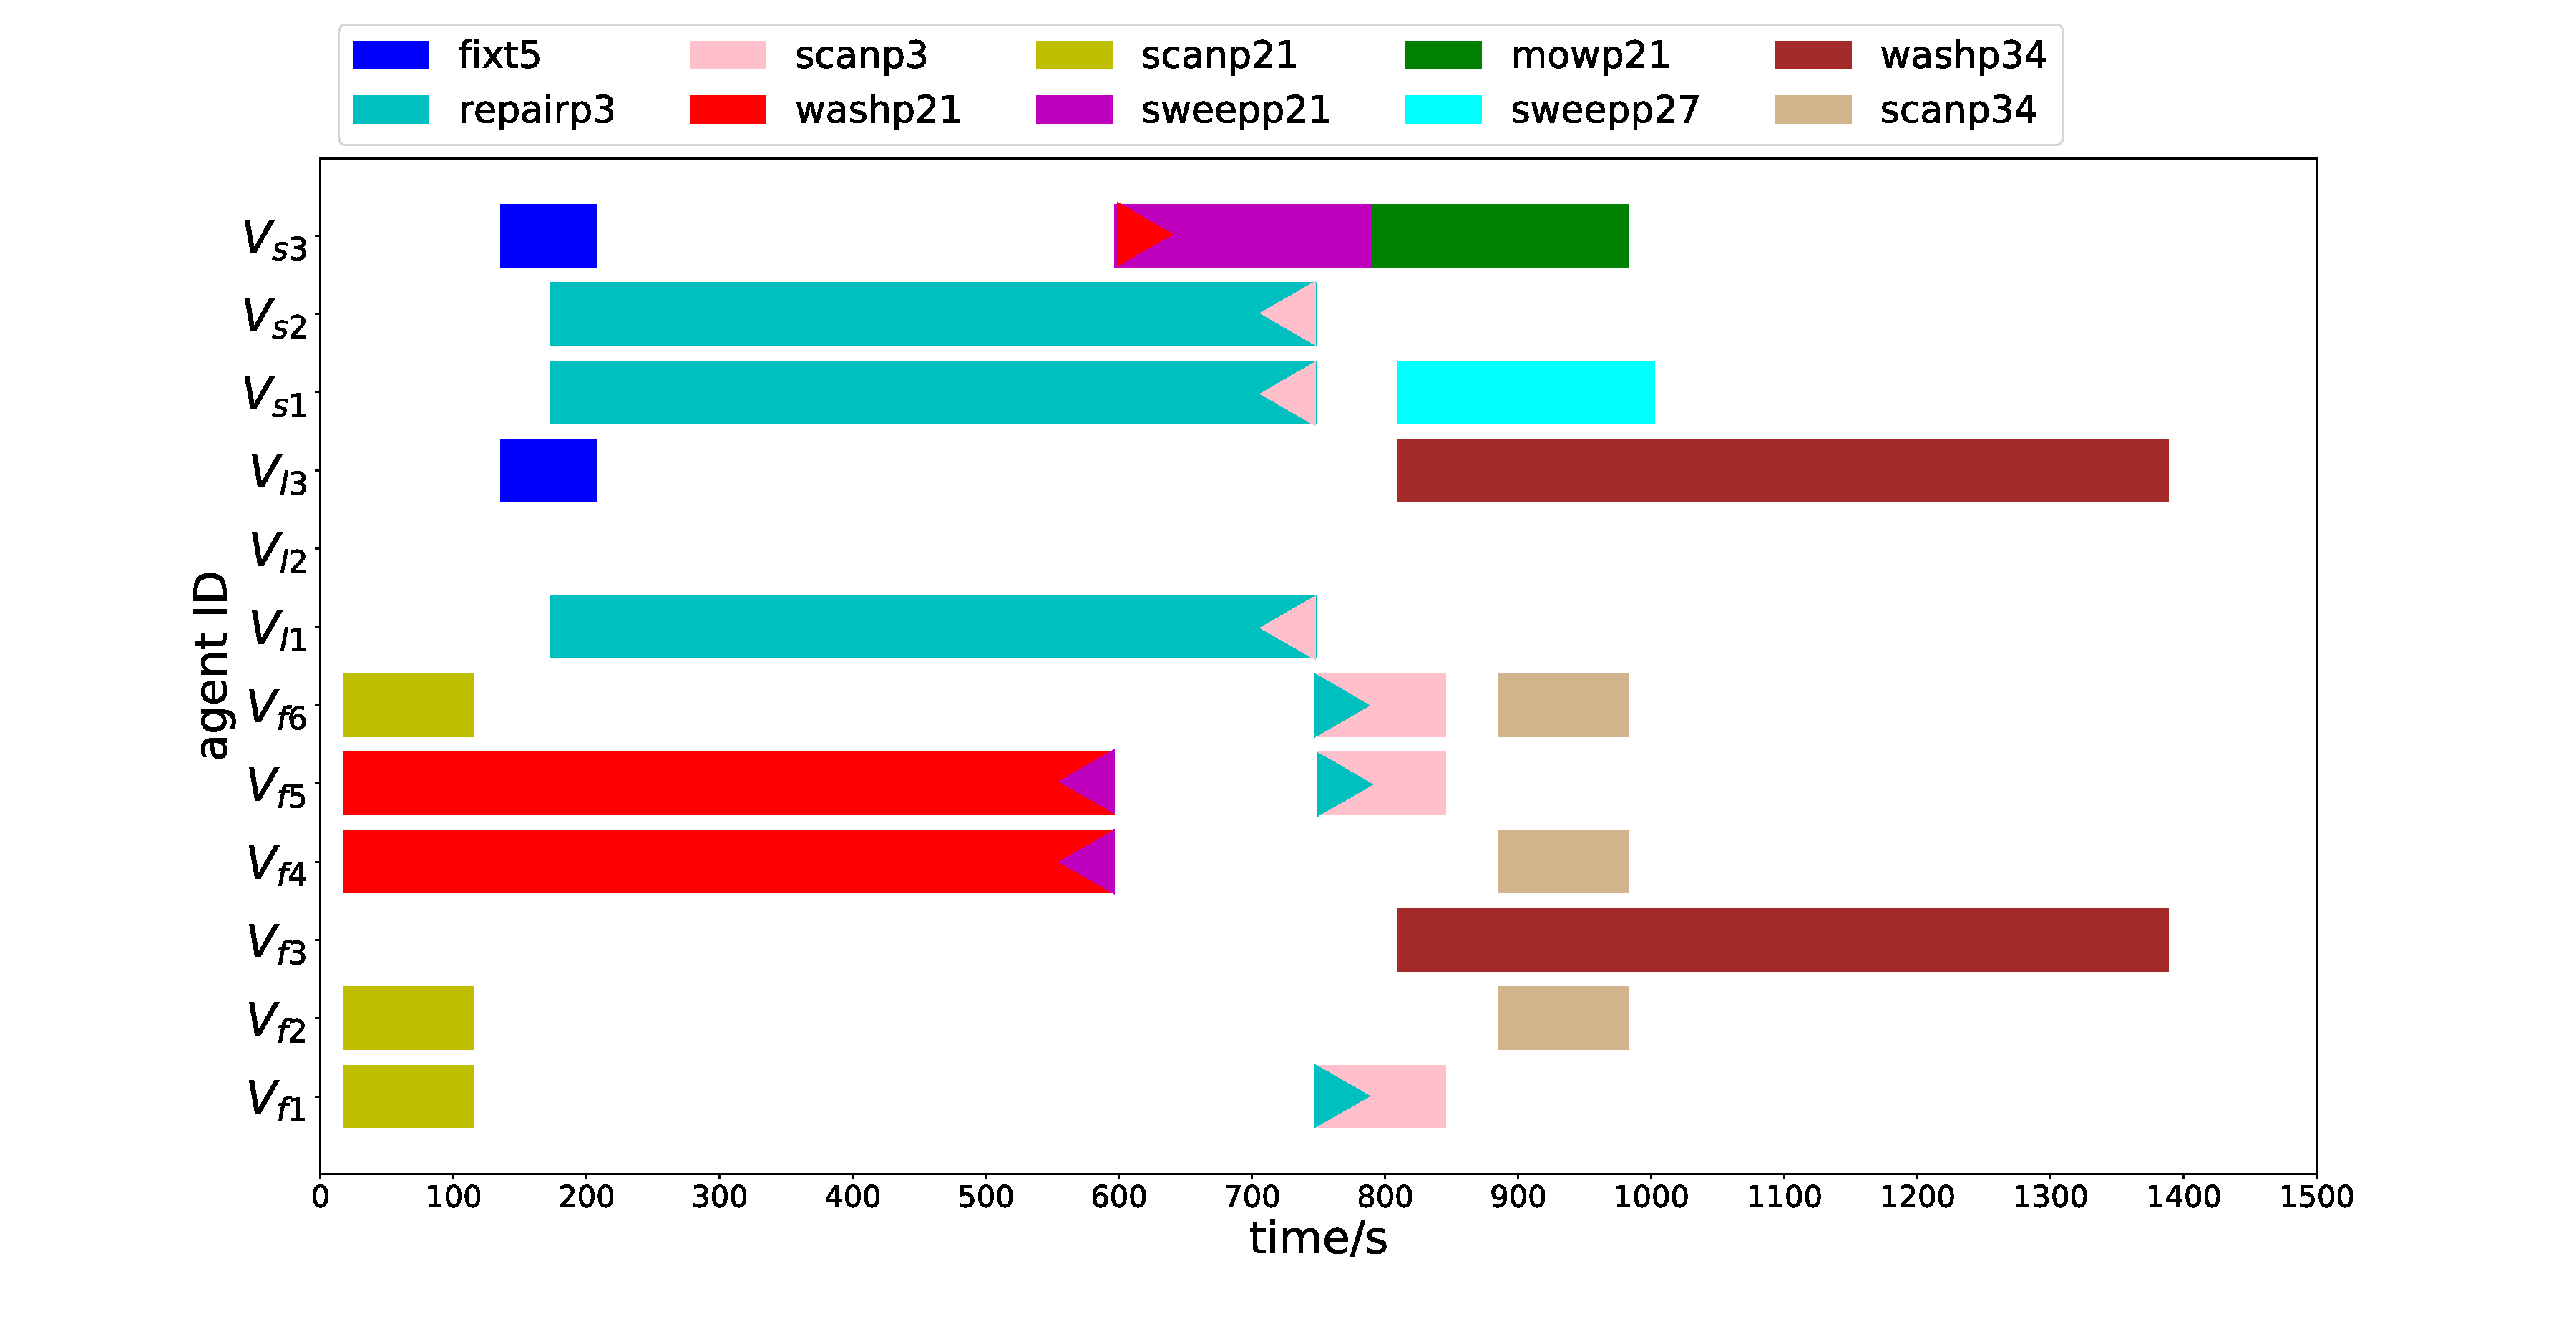
\includegraphics[height =0.5\textwidth]{figures/simulation/taskfinal/gantt_sim.pdf}
	
\end{minipage}%

\begin{minipage}[t]{1\linewidth}
	\centering
	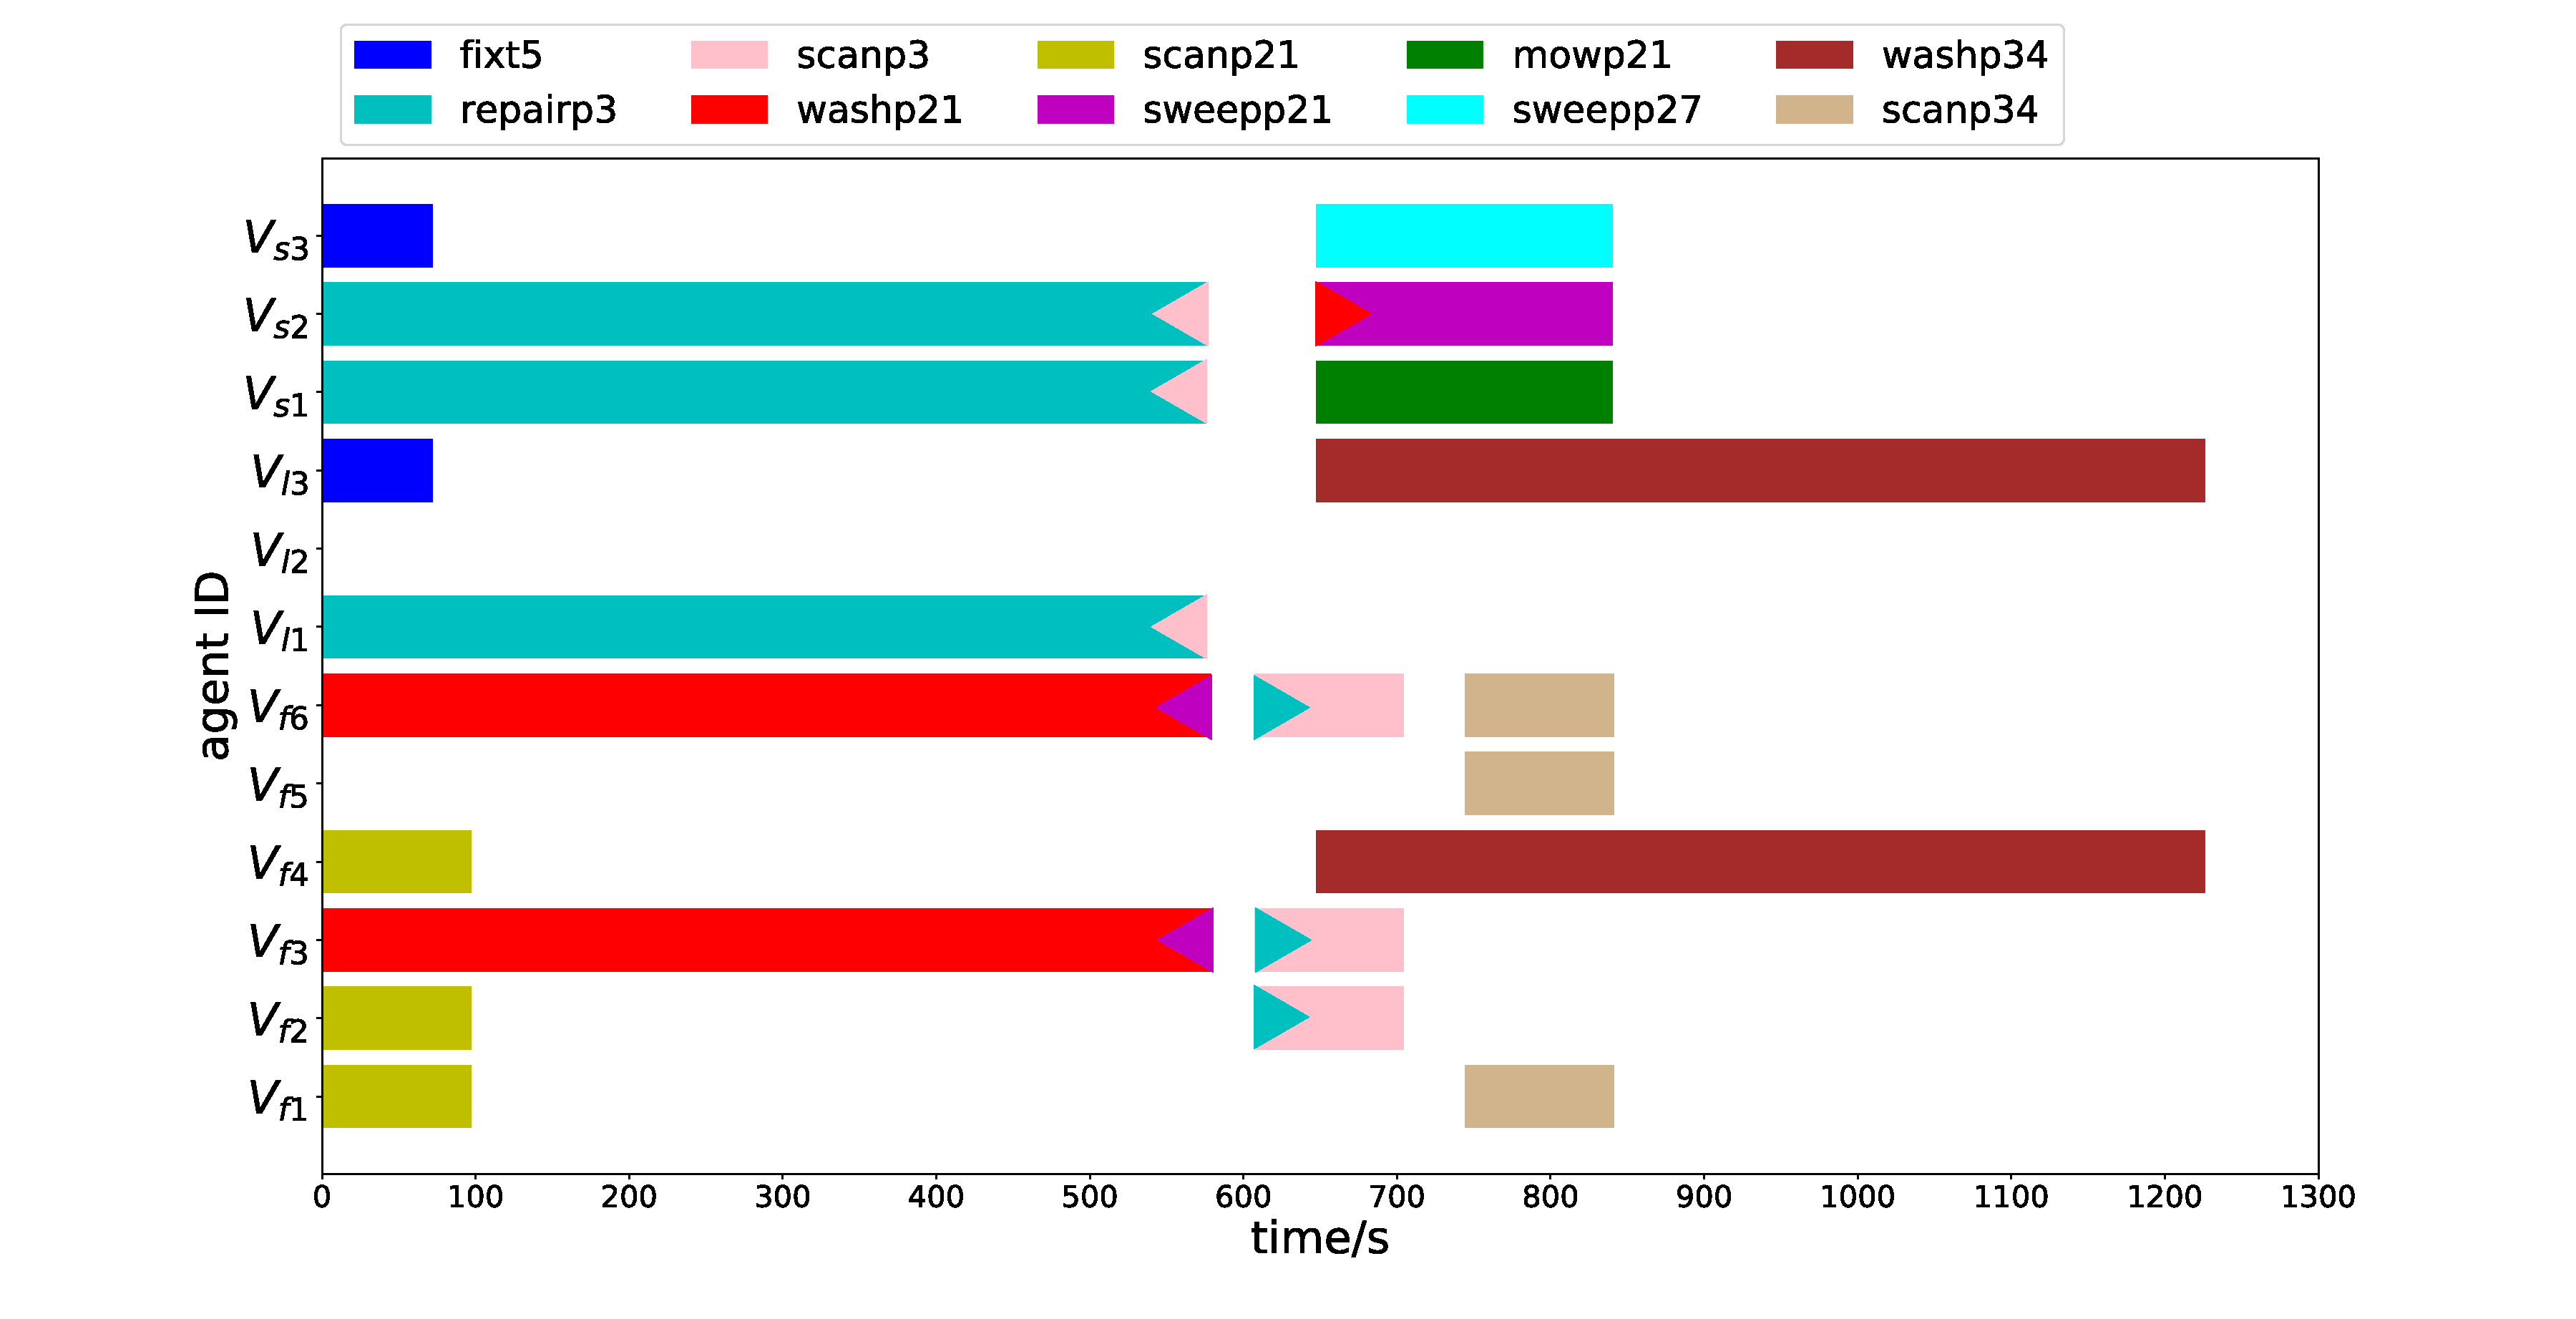
\includegraphics[width =1\textwidth]{ figures/simulation/taskfinal/gantt_graph_suffix.pdf}
\end{minipage}%
   \centering %
   \label{Gantt_graph}
\caption{\textbf{Upper}: Gantt graph of prefix situation. \textbf{Lower}: Gantt graph of suffix situation. } 
\end{figure}
%==============================

%==============================
\subsubsection{Online Adaptation}\label{subsubsec:exp-adapt}
As an important part of the contribution, we now simulate
the following two practical scenarios to validate the proposed online adaptation algorithm.:
(i) fluctuations in the execution time of subtasks;
(ii) several agents break down during the online execution,

First of all, we artificially change the executing time of certain subtasks.
For instance, the executing time of the maintenance tasks for smaller panels
is reduced in comparison to the large panels, e.g., the execution time
of $\texttt{wash}_{\texttt{p}_{34}}$ are reduced to $141s$ from $565s$, as the size
of $\texttt{p}_{34}$ is $25\%$ of~$\texttt{p}_{10}$. And the transfer time 
between different regions will be disturbed.The proposed online synchronization method in
 Sec.~\ref{subsubsec:uncertain} is applied during execution to dynamically accommodate these fluctuations.
As the fig~\ref{fig:online-failure-task} showed, $V_{s_1}, V_{s_2}$ arrived $p_3$ first
and then began "waiting for collaborators" until $V_l1$ arrive $p_3$ and start to executing
  $\texttt{repair}_{\texttt{p}_3}$. And after finished task $\texttt{scan}_{\texttt{p}_{21}}$,
  agent $V_{f_2},V_{f_6}$ go to proper place quickly but cannot start $\texttt{scan}_{\texttt{p}_3}$
  until $\texttt{repair}_{\texttt{p}_3}$ finished. Thus, they turn to the state of "waiting for preceding subtasks
  in partial order".



 
%==============================
\begin{figure}[t]
	  \begin{minipage}[t]{1\linewidth}
		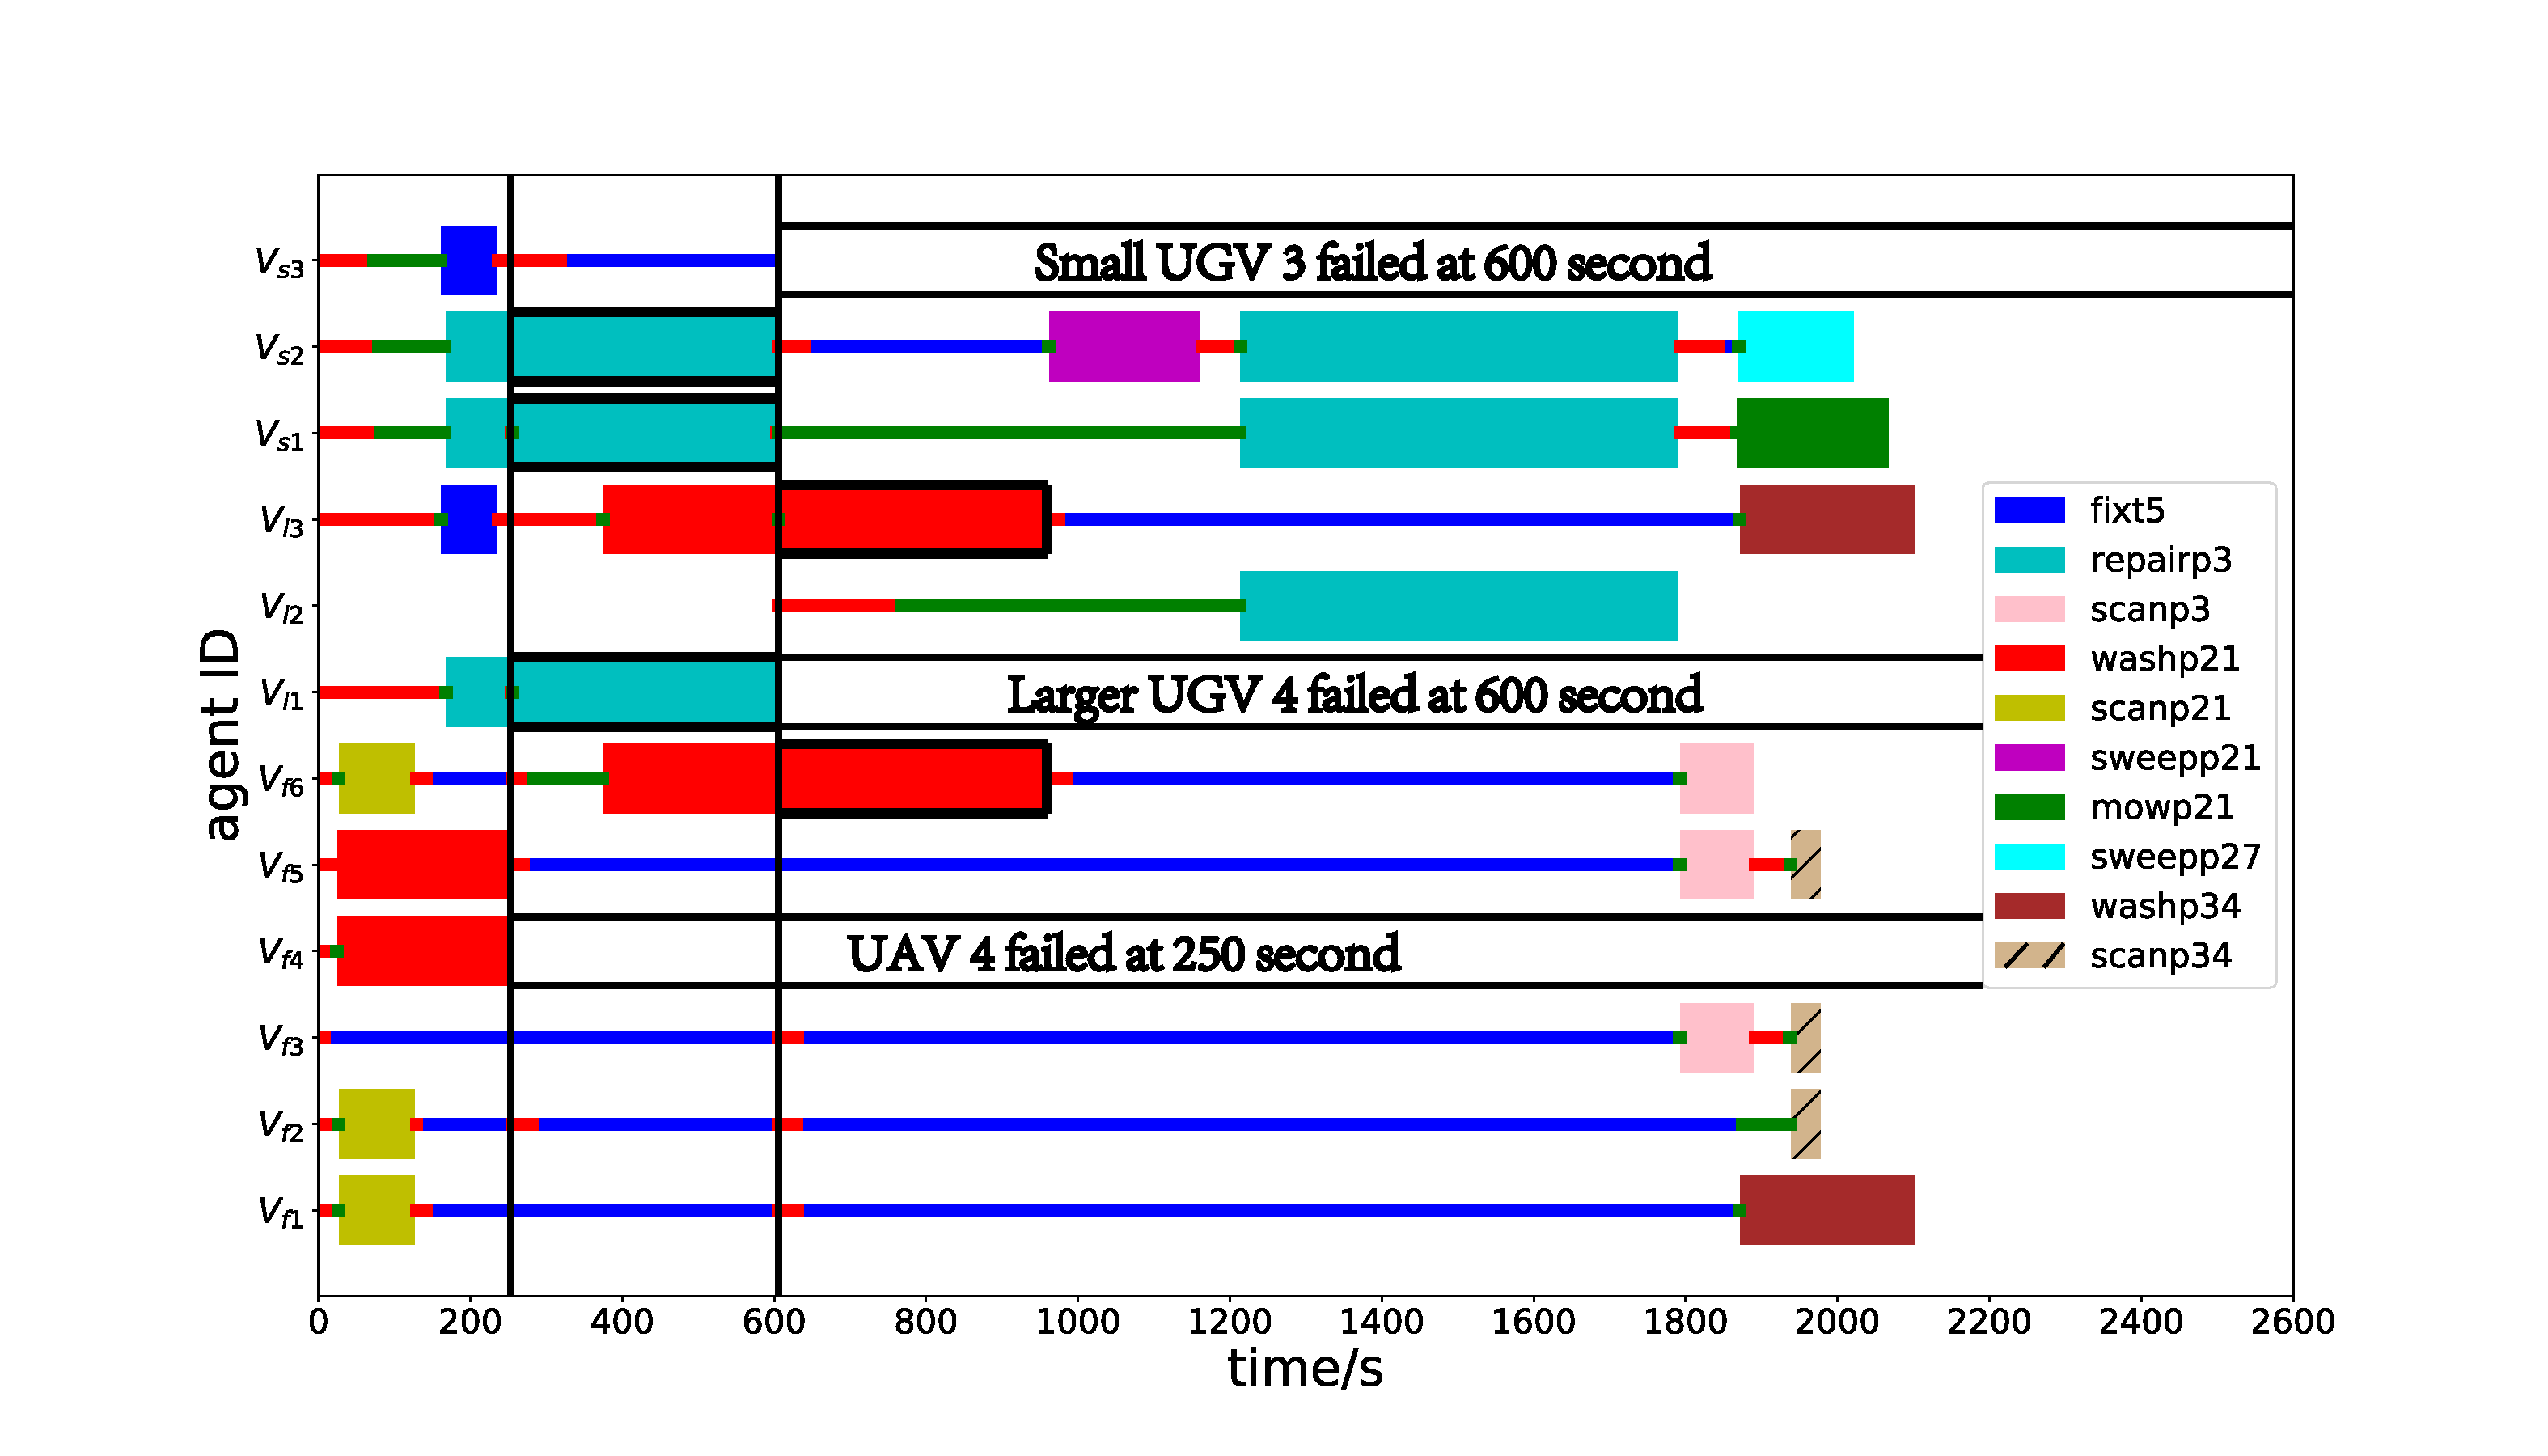
\includegraphics[height =0.6\textwidth]{figures/simulation/taskfinal/gantt_online_prefix.pdf}
	\end{minipage}%
	
	\begin{minipage}[t]{1\linewidth}
		\centering
		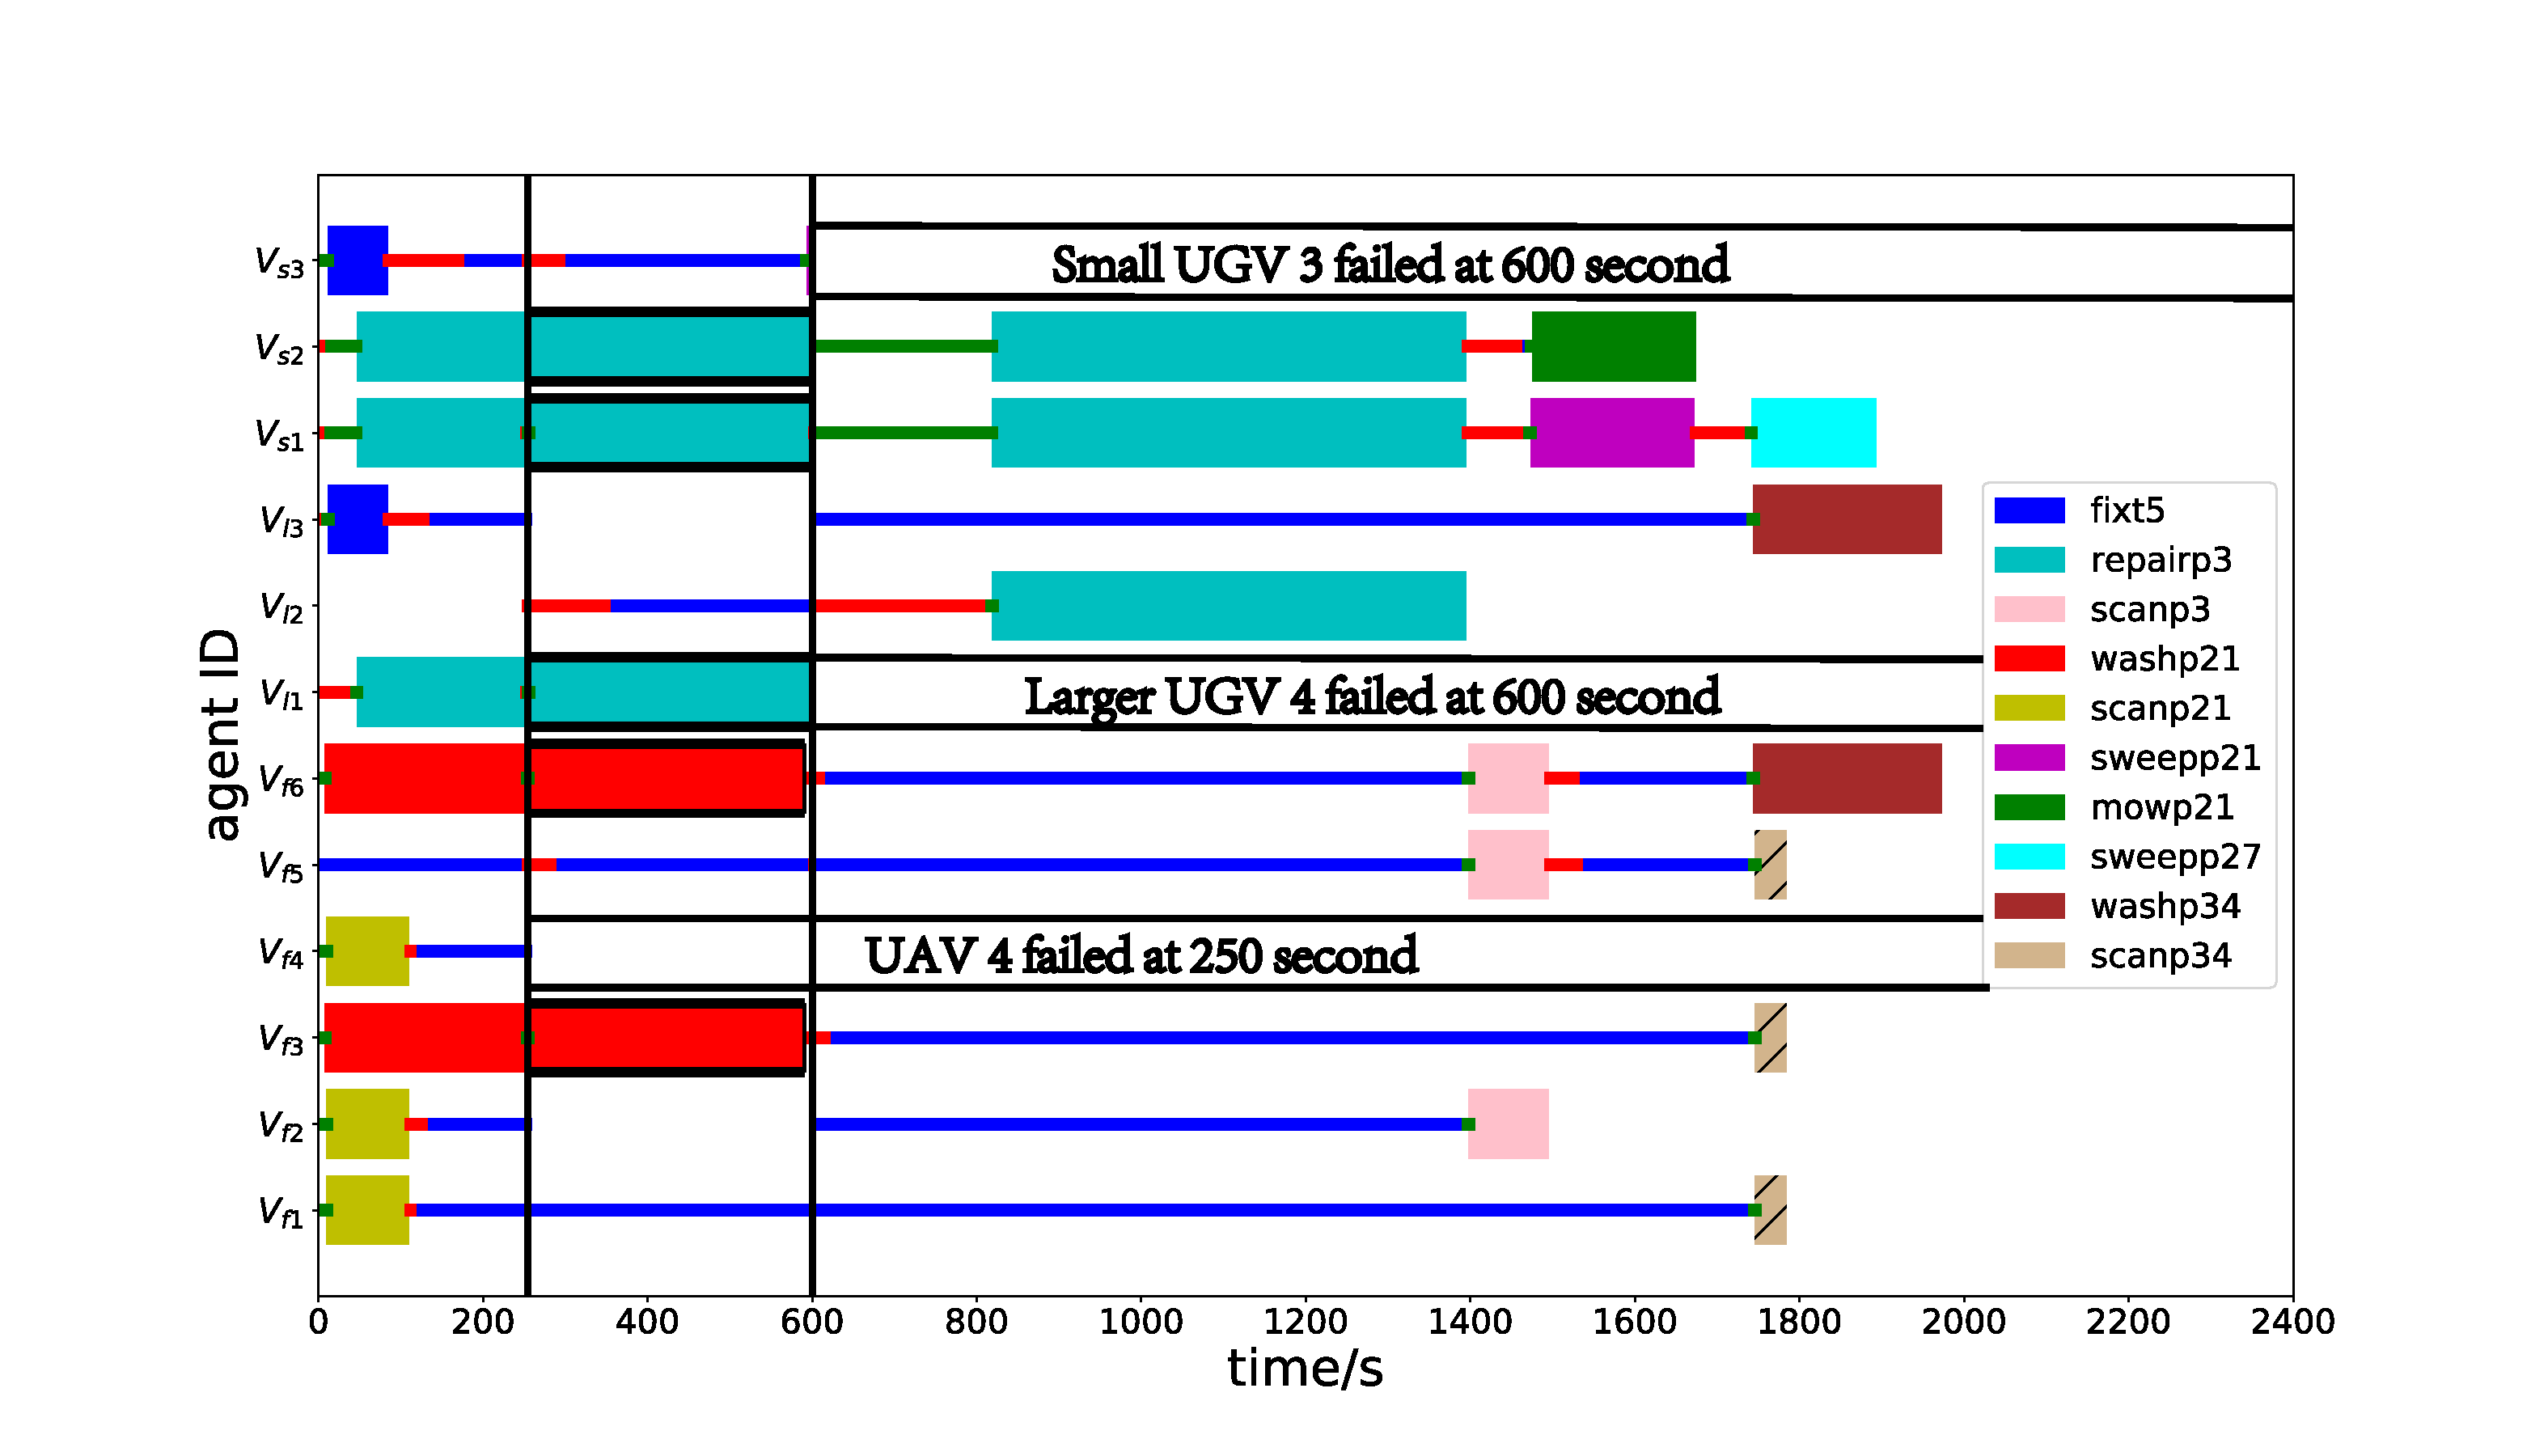
\includegraphics[width =1.05\textwidth]{ figures/simulation/taskfinal/gantt_online_suffix.pdf}
	\end{minipage}%
	\centering
	\caption{
Gantt graph of the plan execution under agent failures and fluctuated subtask duration during the execution.
Additional lines are added to highlight the online synchronization process. Red seqments indicate that the agents
are during transition among regions, green seqments for "waiting for collaborators", and blue segments for 
“waiting for preceding subtask in partial order”. What's more, three failures agent are highlighted in black.
Interrupted subtasks are repeated in the new-assignment.\textbf{Upper}: prefix;\textbf{Lower}:suffix.}
        \label{fig:online-failure-task}
\end{figure}
%==============================


Secondly, more severe scenarios are simulated where agents break down
during task execution and thus are removed from the team.
More specifically, vehicle~$V_{f_3}$ breaks down at~$200s$, $V_{l_1},\, V_{s_3}$ break
down at~$600s$ during the execution of $\varphi_1$.
Consequently, as shown in Fig.~\ref{fig:online-failure-task}, $\texttt{wash}_{\texttt{p}_{21}}$
is re-assigned to other agent as one of its cooperaters $V_{f_3}$ is failed. And subtask 
$\texttt{repair}_{\texttt{p}_{3}}$ is continuing as its cooperate situation and partial relations 
are still satisfied. As described in Sec.~\ref{subsubsec:failure},
the set of unfinished tasks is re-assigned to the remaining agents by re-identifying
the current node in the BnB search tree and continue the planning process.
It can be seen that no subtasks are assigned to~$V_{f_3}$ anymore in the updated assignment.
Then, as $V_{l_1},\, V_{s_3}$ break down at $600s$, the execution of subtask~$\texttt{repair}_{\texttt{p}_{3}}$ 
is interrupted. And it is executed again by vehicles~$V_{l_2}$ and $V_{s_1},V_{s_3}$ at~$1222s$.
In the same way, the unfinished subtasks are re-assigned to the remaining agents.
It is worth noting that the partial ordering constraints are respected at all
time during the adaptation.
For instance, $V_{f_1}$ cannot execute the subtask~$\texttt{wash}_{\texttt{t}_{34}}$
before~$\texttt{mow}_{\texttt{p}_{21}}$ is started,
as~$\texttt{mow}_{\texttt{p}_{21}}\leq_\varphi\texttt{wash}_{\texttt{p}_{34}}  $ holds.
All subtasks are fulfilled at~$2109s$, despite of the above contingencies.
So does the situation of suffix.


%==============================
\subsubsection{Scalability Analysis}\label{subsubsec:scalable}
To further validate the scalability of the proposed methods,
the following tests are performed:
(i) the same task with increased team sizes,
e.g., $16$, $24$, $32$ and $40$;
(ii) test more LTL formula list with different structure. 

As summarized in Table~\ref{table:more-agents},
as the system size is increased from~$8$ to $40$,
the computation time to obtain the \emph{first}
solution for task Three remains almost unchanged,
while the time taken to compute the optimal value increases slightly.
This result verifies that the proposed anytime algorithm is beneficial
especially for large-scale systems, as it can returns a high quality solution fast,
and close-to-optimal solutions can be returned as time permits.
Secondly, more tasks as $\varphi_2,\varphi_3$ are considered as follows:
\begin{equation}\label{eq:task2}
\begin{aligned}
\varphi_2 = &\Diamond (\texttt{wash}_{\texttt{p}_{11}} \land \lnot\texttt{scan}_{\texttt{p}_i} 
\wedge\Diamond \texttt{scan}_{\texttt{p}_{11}}\wedge \Diamond ((\texttt{mow}_{\texttt{p}_{11}}\\
&\wedge\lnot \texttt{wash}_{\texttt{p}_{11}} ) \wedge\Diamond (\texttt{sweep}_{\texttt{p}_{11}} \land \lnot\texttt{mow}_{\texttt{p}_{11}} )))\\
&\Diamond (\texttt{temp}_{\texttt{p}_{25}} \land \Diamond \texttt{repair}_{\texttt{p}_{25}}\wedge \Diamond ((\texttt{scan}_{\texttt{p}_{25}}\wedge\\
&\lnot \texttt{wash}_{\texttt{p}_{25}} ) \wedge\Diamond (\texttt{sweep}_{\texttt{p}_{25}} \land \lnot{\texttt{p}_{26}} ))) \wedge  \Diamond
\texttt{temp}_{\texttt{t}_4},
\end{aligned}
\end{equation}  

\begin{equation}\label{eq:task3}
\begin{aligned}
\varphi_3 = &\Diamond (\texttt{temp}_{\texttt{p}_{25}} \land\Diamond \texttt{repair}_{\texttt{p}_{25}}\wedge \Diamond ((\texttt{scan}_{\texttt{p}_{25}}\wedge\\
&\lnot \texttt{wash}_{\texttt{p}_{25}} ) \wedge\Diamond (\texttt{sweep}_{\texttt{p}_{25}} \land \lnot{\texttt{p}_{26}} ))) \wedge  \Diamond
\texttt{temp}_{\texttt{t}_4},\\
&\wedge  \Diamond (\texttt{sweep}_{\texttt{p}_{8}} \wedge \Diamond \texttt{wash}_{\texttt{p}_{8}} )\land \Diamond \texttt{repair}_{\texttt{p}_4} \bigcirc \lnot \texttt{p}_4\\
& \wedge \Diamond ( \texttt{sweep}_{\texttt{p}_{8}} \wedge \lnot \texttt{wash}_{\texttt{p}_{8}} \wedge\Diamond \texttt{scan}_{\texttt{p}_{8}} )\\ 
&\wedge \lnot \texttt{temp}_{\texttt{t}_4} \,U \, \texttt{fix}_{\texttt{t}_{4}},
\end{aligned}
\end{equation}
where~$\mathcal{B}_{\varphi_2}$ contains $216$ state
	 and~$\mathcal{B}_{\varphi_3}$ contains~$970$ state.
	As summarized in Table~\ref{table:more-agents} , the computation time of
	 both posets and tasks assignment are increased significantly, as the task becomes more
	 complex. 
	 However, the time when the first solution is obtained in tasks assignment does not monotonically increase due to
	 the polynomial complexity of upper bound method. }
 


%==============================
\begin{table}[t]
  \centering
  \begin{threeparttable}
	\caption{Scalability analyses of the proposed method}
	\label{table:more-agents}
  \begin{tabular}{|c|c|c|c|}\hline
    \tnote{1} \begin{tabular}{@{}c@{}} System \\ $(V_f,V_s,V_l)$\end{tabular}
    &  \tnote{3} $t_{\varphi_1}\,[s]$
    &  $t_{\varphi_2}\,[s]$
    & \tnote{3} $t_{\varphi_3}\,[s]$  \\[0.5ex] \hline 
		$(8,4,4)$ & $0.13,5.9$ &$0.14,1.08$ & $0.23,4.81$  \\[0.5ex]
		$(12,6,6)$ & $0.15,4.6$  & $0.08,1.85$ & $0.22,5.23$ \\[0.5ex]
		$(16,8,8)$  & $0.13,5.0$  & $0.10,1.56$ & $0.21,4.33$ \\[0.5ex]
		$(20,10,10)$  & $0.53,8.4$ & $0.09,2.11$ & $0.58,6.20$  \\[0.5ex] \hline
		\tnote{2} Poset analysis  & $64.4,71.1$ &$8.4,37.9$ & $136.4,552.5$ \\ [0.5ex]
    \hline
  \end{tabular}
  \begin{tablenotes}
    \item[1] The number of different types of agents as system size increases.
    \item[2] The associated solution time, measured by two time stemps when: the
    first poset is returned, the best poset with largest language is returned.
    \item[3] The associated solution time,
          measured by two time stamps when:
          the first solution is returned,
          and the optimal solution is returned.
  \end{tablenotes}
\end{threeparttable}
\end{table}
%==============================

%==============================
\subsubsection{Comparison}\label{subsubsec:compare}
The proposed method is compared against several
state-of-the-art methods in the literature.
More specifically, four methods below are compared:

\textbf{Prod}: the standard solution~\cite{baier2008principles}
that first computes
the Cartesian products of all agent models,
then computes the product B\"uchi automaton,
and searches for the accepting run within.
As the brute-force method,
it is well-known to suffer from complexity explosion.

\textbf{Milp}: the optimization-based solution that
formulates the assignment problem of posets as a MILP
the compute optimal assignment similar
to~\cite{luo2021temporal, jones2019scratchs},
i.e., instead of the search method.
The partial relations are formulated as constraints
in the program.
An open source solver GLPK~\cite{makhorin2008glpk} is used.

\textbf{Samp}: the sampling based method proposed
in~\cite{kantaros2020stylus}.
Compared with the product-based methods, it does not pre-compute
the complete system model. Instead it relies on a sampling strategy
to explore only relevant search space.
However, since it does not support collaborative actions natively,
we modify the definition of transitions there slightly.

\textbf{Decomp}: the task assignment strategy proposed
in~\cite{schillinger2018simultaneous}.
As discussed earlier in Sec.~\ref{sec:introduction},
the proposed task decomposition strategy only allows completely
independent subtasks.
Furthermore, since it does not support collaborative actions,
collaborative subtasks are decomposed manually.
%==============================
\begin{table}[t]
  \centering
  \begin{threeparttable}
	\caption{Comparison to other methods.}
	\label{table:compare}
	\begin{tabular}{|c|c|c|c|c|c|}\hline
	  \tnote{1} Method & \tnote{2} $t_{\texttt{first}}\, [s]$
          & \tnote{2} $t_{\texttt{opt}}\, [s]$
	  & \tnote{2} $t_{\texttt{final}}\,[s]$ & \tnote{2} $T_{\texttt{obj}}\,[s]$
          & \tnote{2} $N_{\texttt{sync}}$ \\[0.5ex] \hline
		\multirow{2}{*}{\textbf{Prod}}& $\infty$ & $\infty$ & $\infty$ & -- & -- \\[0.5ex]
                 & $\infty$ & $\infty$ & $\infty$ & -- & -- \\[0.5ex]
                \hline
		\multirow{2}{*}{\textbf{Milp}} & 2069.27 & 2069.27 & 2069.27 & 1058.47 & -- \\[0.5ex]
                &$\infty$ &$\infty$ & $\infty$ & -- & --  \\[0.5ex]
                \hline
		\multirow{2}{*}{\textbf{Samp}} & 328.59 & 1838.96 & $\infty$ & 1968.03 & 24 \\[0.5ex]
                 & 3280.68 &  16294.30 & $\infty$ & 1968.03 & 24 \\[0.5ex]
                \hline
		\multirow{2}{*}{\textbf{Decomp}} & 580.16 & 580.16 & 4581.3 & 1266.99 & 0 \\[0.5ex]
		 & 1151.24 & 1151.24 & 5082.07 & 1267.00 & 0 \\[0.5ex]
                \hline
		\multirow{2}{*}{\textbf{Ours}} & 24.81 & 25.26 & $\infty$ & 1058.47 & 8 \\[0.5ex]
                 & 28.12 & 37.40 & $\infty$ & 1058.47 & 8 \\[0.5ex]
		\hline
	\end{tabular}
  \begin{tablenotes}
  \item[1] For each method, the first row measures the time for the
    system of~$12$ agents while the second row for~$24$ agents.
  \item[2] The time to derive the first solution,
    the time to derive the optimal solution,
    the termination time, the objective as the task completion time,
and the number of synchronizations required.
  \end{tablenotes}
   \end{threeparttable}
\end{table}
%==============================

Two identical comparisons are performed under different system sizes,
namely $12$ and $24$ agents, to compare not only efficiency but also scalability.
To begin with, the nominal system of~$12$ agents under task~$\varphi_2$ is considered.
The above four methods are used to solve the same planning problem.
As summarized in Table.~\ref{table:compare},
the results are compared in the following four aspects:
the time to derive the first solution,
the time to derive the optimal solution,
the termination time, the optimal solution,
and finally the number of online synchronizations required.
Since the methods \textbf{Prod}, \textbf{Milp} and \textbf{Decomp} are not
anytime, the time to obtain  the first solution equals to the time
when the optimal solution is obtained.
It can be seen that the \textbf{Prod} failed to generate any solution
within~$11h$ as the system-wide product automaton for both cases
has more than $10^{19}$ states.
The \textbf{Milp} method is only applicable for small problems,
which returns the optimal solution in~$0.5h$ but fails to
return any solution within~$16h$ for the large problem.
The \textbf{Samp} method has the anytime property but it takes ten times
the time to generate
the first feasible solution, compared with our method.
In addition, since the subtasks are executed in sequence by the solution,
the actual time of task completion is significantly longer.
The \textbf{Decomp} method can solve both problems but the overall time
for task completion is longer than our results,
which matches our analyses in Remark~\ref{remark:compare-poset}.
In comparison, our method returns the first solution for both cases in less
than~$30s$ and the optimal solution within another~$10s$.
It can be seen that the task completion time remains the same for both cases,
which is consistent with the \textbf{Milp} method.

Last but not least, the last column in Table~\ref{table:compare} compares the number
of synchronizations required during execution.
Although the same solution is obtained, the \textbf{Milp} method requires more
synchronization during execution than our method.
This is because our method requires only synchronization for relations within the
posets, rather than all consecutive subtasks.
The \textbf{Prod} and \textbf{Samp} methods require more synchronization due to
its fully sequential execution,
while the \textbf{Decomp} requires no synchronization as
the local subtasks of each agent are independent.
